\subsection{Leksikalsk analyse}
\begin{frame}
  \frametitle{Leksikalsk analyse}

  \begin{itemize}
    \item Lexemes $\rightarrow$ Tokens
    \item Ingen specific syntaks
    \item $(\mathbf{Type}\; \mathrm{tokenType},\; \mathbf{String}\;
      \mathrm{value},\; \mathbf{int}\; \mathrm{line},\; \mathbf{int}\;
      \mathrm{offset})$
  \end{itemize}

\end{frame}

\begin{frame}
  \frametitle{Leksikalsk analyse}

  \begin{figure}
    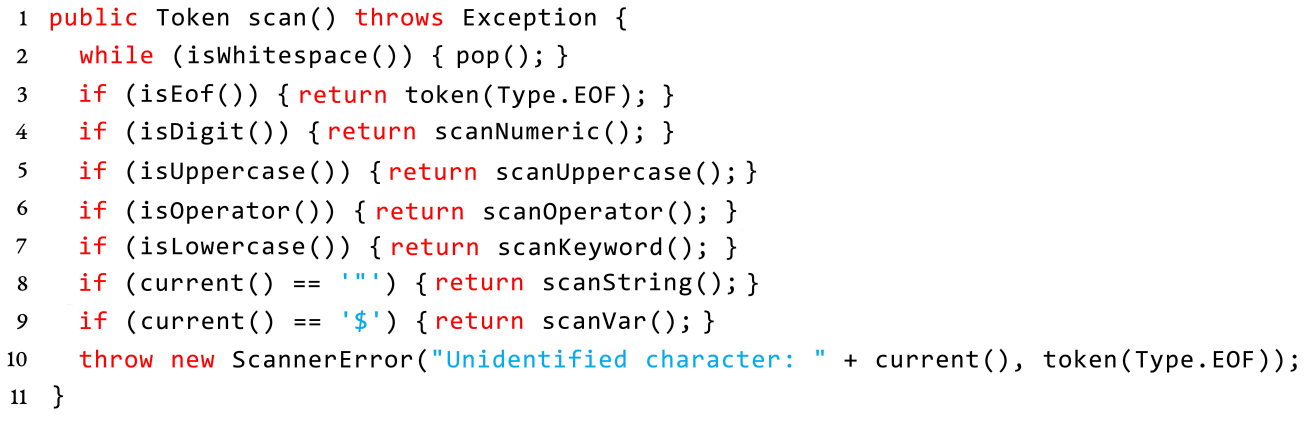
\includegraphics[width=1\linewidth]{billeder/scan-metode}
  \end{figure}

\end{frame}



\begin{frame}
  \frametitle{Leksikalsk analyse}

  \begin{figure}
    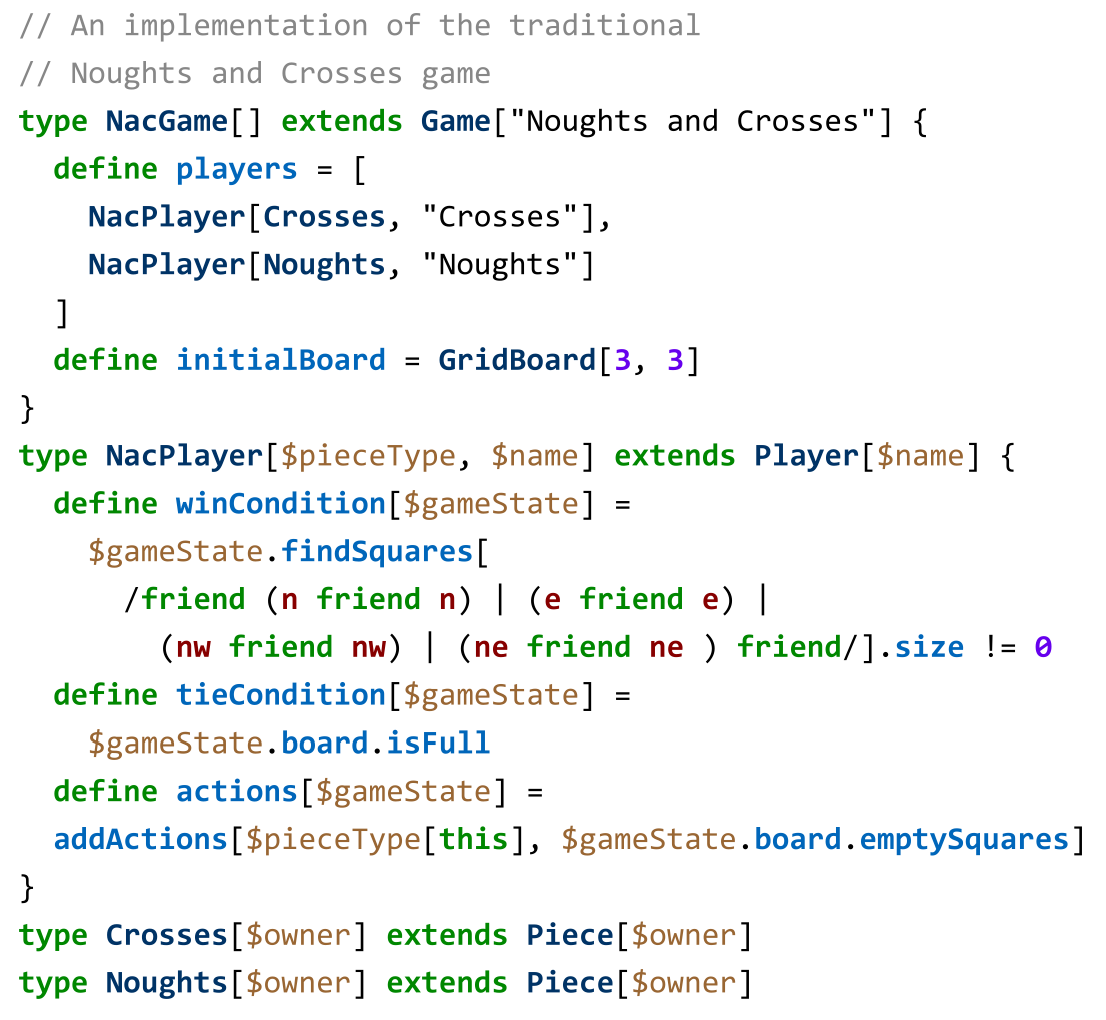
\includegraphics[width=0.6\linewidth]{billeder/leksikalsk-eksempel}
  \end{figure}

\end{frame}

